% This is samplepaper.tex, a sample chapter demonstrating the
% LLNCS macro package for Springer Computer Science proceedings;
% Version 2.20 of 2017/10/04
%
\documentclass[runningheads]{llncs}
%
\usepackage{graphicx}
\usepackage{booktabs}
\usepackage{multirow}
% Used for displaying a sample figure. If possible, figure files should
% be included in EPS format.
%
% If you use the hyperref package, please uncomment the following line
% to display URLs in blue roman font according to Springer's eBook style:
% \renewcommand\UrlFont{\color{blue}\rmfamily}

\begin{document}
%
\title{Water Quality Modeling and Prediction Method Based on Sparse Recurrent Neural Network\thanks{This work is supported by Public Projects of Zhejiang Province (2016C31G2020069) and the 3rd Level in Zhejiang Province “151 talents project” to Zhenbo Cheng.}}
%
%\titlerunning{Abbreviated paper title}
% If the paper title is too long for the running head, you can set
% an abbreviated paper title here
%
\author{Zhenbo Cheng\inst{} \and
Zhengyuan Shen\inst{} \and
Tianqi Zhu\inst{}\and
Huaidi Lin\inst{}\and
Leilei Zhang\inst{}}
%
\authorrunning{Z.B. Cheng et al.}
% First names are abbreviated in the running head.
% If there are more than two authors, 'et al.' is used.
%
\institute{Zhejiang University of Technology, Hangzhou, China \\
\email{czb@zjut.edu.cn}}
%
\maketitle              % typeset the header of the contribution
%
\begin{abstract}
It is an important prerequisite for scientific management and maintenance of water 
resources to accurately predict all kinds of indicators that affect water quality. 
This paper proposed a method of forecasting water quality index and rank based on sparse 
recurrent neural network (SRNN). Based on the principle of minimum mean square 
recursive error, the training algorithm of the network was designed. The neural network was used to construct a water quality prediction model. The experimental results showed that the model can be used to predict the 
 trend of water quality in ZheJiang province.


\keywords{Water quality modeling\and Water quality prediction\and Recurrent neural network.}
\end{abstract}
%
%
%

\section{Introduction}
With the rapid economic development and population growth, 
sewage and wastewater generated by the production and living of 
human are posing a serious threat to the water quality of lakes and 
rivers\cite{RN1}.There are various problems such as water shortage, water 
pollution and deterioration of water ecological environment in all 
parts of China\cite{RN1}, which has become the main bottleneck restricting the 
sustainable development of economy and society. In order to effectively solve this problem, the rational planning 
of water resources is particularly important\cite{RN2,RN3}. Accurate detection of water 
quality parameters of rivers and lakes, as well as reasonable prediction
of future changes in water quality parameters\cite{RN4}, is a necessary 
prerequisite for scientific planning of water resources. Water quality 
prediction is the process of constructing a water quality model using 
existing data and then estimating the future water quality parameters of 
the predicted point via the model. Common predictive models can be divided 
into two categories: Principle Driven Model (PDM) and Data Driven Model (DDM).

PDM is generally based on the principle of mass and energy conservation, 
and considers the interaction between water quality components and its
own biochemical effects, and then through the construction of hydrodynamic 
motion and energy equations of water\cite{RN5,RN6}. Typical principle driven water 
quality models include the Streeter Phelps(SP) model for quantifying oxygen 
balance\cite{RN7}, which is often applied to simple water body self-purification; 
a QUAL model capable of simulating up to 15 water quality components\cite{RN5}, 
which is often used to study the impact of influent wastewater load on the water 
quality of the receiving river; the Water Quality Analysis Simulation Program(WASP) 
model of pollutant interaction\cite{RN6} and the BASINS model combined with geographic 
information system\cite{RN5,RN8}. The above prediction model has been widely used 
in water pollution control and early warning, water quality planning and 
other fields because it can accurately describe the relationship between 
various components of water. For PMD, however, once the factors affecting 
water quality change, it is often necessary for domain experts to redesign 
the model, resulting in the lack of flexibility in the application of 
such water quality models.

The construction of DDM which is different from PDM does not necessarily 
require the participation of domain experts. It only needs to input 
a large amount of water quality data into a learning model, and then 
adjust the parameters of the learning model according to the algorithm 
to obtain the mapping between the input data and the data to 
be predicted. The learning model with adjusted parameters can be 
used for water quality prediction. Common learning models include various 
regression analysis based on statistical principles\cite{RN9,RN10,RN11,RN12} and artificial
neural network (ANN)\cite{RN13,RN14,RN15,RN16,RN17,RN18}. Because these models have a learning process, they can be applied to various water quality predictions under environmentally variable scenarios.

In order to obtain higher prediction accuracy, the ANN 
commonly used in DDM often needs a large number of historical 
water quality data, and then automatically learns the water 
quality prediction model to meet the demand according 
to the historical data. However, the back propagation (BP) 
network which is commonly used in ANN often has the 
disadvantage of slow convergence speed. In addition, BP network is 
a typical feedforward structure neural network, but water quality data 
is often a time series\cite{RN19}. BP network is difficult to simulate the time 
correlation between water quality data. Therefore, based on the latest theoretical research results of the prefrontal cortex in neuroscience\cite{RN20,RN21}, this study quickly constructs a model between water quality data through a recursive least mean square error algorithm by constructing a sparsely connected large-scale recurrent neural network. The accuracy of the model was verified by predicting the water quality 
 indicators such as ammonia nitrogen (AN), dissolved oxygen (DO), permanganate index (PI), 
 total phosphorus (TP) and total nitrogen (TN) in a river.
\section{Water quality model}
This study used a sparsely connected recurrent neural network (SRNN)
to simulate the temporal correlation between water quality data. 
SRNN which is unlike common recurrent neural networks contains a 
large number of neurons. The positive and negative connection 
weights between neurons are roughly the same. In particular, 
when the intensity coefficient of weighted connections between 
neurons in SRNN exceeds a certain threshold, the spontaneous activity 
of the recursive network will exhibit chaotic characteristics\cite{RN17}. 
This feature makes the network have strong state coding capabilities. 
SRNN has been widely used in cognitive modeling of neuroscience. 
Some theoretical neuroscientists even speculate that SRNN is similar 
to the function of the prefrontal cortex of the brain\cite{RN18}.
\subsection{SRNN network structure}
As shown in Figure \ref{Structure of SRNN}, 
the SRNN contains three parts, an input layer y, a recursive layer x, and an output layer z.
Vector y =$\left[y_1,y_2,...,y_m\right]^T$ represents the input layer neuron activity,
 where $y_i$ is the input water quality indicator and the superscript T is the transpose.

\begin{figure}[htbp]
\centering
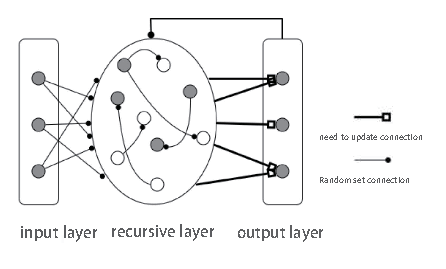
\includegraphics[width=\columnwidth]{Structure_of_SRNN}
\caption{Structure of SRNN}
\label{Structure of SRNN}
\end{figure}

Neuronal activity level is represented by recursion x, 
whose activity was calculated by the formula:

\begin{equation}
\tau \frac{d_x}{d_t}=-x+w^{RNL}r+w^{in}y+w^{fb}z,
\end{equation}
where $r = \tanh(x)$represents the rate of release 
of recurrent layer neurons and tanh is a hyperbolic 
tangent function as well as the activation function of 
recursive layer neurons. $\tau=0.01$is the neuron activity
 decay constant.

$w^{RNL}$represents the recursive connection matrix between 
neurons in the recursive layer.
Since the recursive layer has $N=1000$ neurons,$w^{RNL}$is a 
matrix of size $1000\times1000$.The element $w_{ij}^{RNL}$
in the matrix represents the connection weight between 
the i-th neuron and the j-th neuron in the recursive layer.
The recursive layer is a sparse connection, and $w_{ij}^{RNL}$
sets the probability of $p=0.1$ to a non-zero value and the 
probability of $1-p=0.9$ to zero.This means that only a few 
of the reciprocal layer neurons have a mutual connection. 
The value of the non-zero element of $w_{ij}^{RNL}$ 
is randomly selected from the Gaussian distribution $Norm(0,g^{2}/pN)$,
where $g$ is the intensity coefficient of weight.
When $g?1.5$, the recursive layer neurons will have the 
spontaneous activity of chaotic characteristics\cite{RN17}.

$w^{in}$ represents the connection matrix between the 
input layer and the recursive layer.
The weights are randomly selected according to the 
Gaussian distribution $Norm(0, 0.5)$.$w^{fb}$ is the connection 
weight of the output neuron feedback back to the layered neuron. 
It is still a sparse connection.90$\%$ of the weights are set to 0, 
and other non-zero elements are still randomly selected according 
to the Gaussian distribution $Norm(0,0.5)$.
z is the output layer neuron activity, corresponding to 
the predicted output, and its calculation is determined by:
\begin{equation}
z=wr
\end{equation}
where $w$ represents the connection matrix between the recursive layer 
and the output layer. The recursive layer and the output layer are 
fully connected, and the weights are randomly assigned according 
to a uniform distribution between $\left[-1,1\right]$. 
$w$ is different from $w^{RNL}$, $w^{in}$, and $w^{fb}$, and
its element values need to be updated during the learning phase,
 while the values of $w^{RNL}$, $w^{in}$, and $w^{fb}$ remain unchanged during 
 the learning phase.

As can be seen from the structure of SRNN, it is similar to the Echo 
State Network (ESN) \cite{RN22}.
They all have a recursive layer and the learning process only adjusts 
the weight between the recursive layer and the output layer. However, 
SRNN and ESN also have the following differences. First of all, 
the SRNN's recursive layer connection weight does not need to be 
specially set, but the ESN needs to have a weight matrix with a 
spectral radius greater than or equal to 1 in order to achieve reverberation.
Secondly, the training of ESN is a kind of offline learning. It needs to wait 
for the network to pre-calculate for a period of time before starting to
adjust the weight, but SRNN can update the weight immediately according 
to the current input.

\subsection{SRNN learning algorithm}
According to the description of SRNN in the previous section, 
the recursive layer connection weights only need to be randomly 
selected according to a given probability distribution and use the 
online learning mode. These features require a learning algorithm 
that quickly determines how the output weight should be 
updated so that the network output is equal to the value of the 
real output.

The target output expected at time $t$ is $f(t)$. The real 
output of the network is $w^T (t-\Delta t) r$.The error between them is $e(t)$.
\begin{equation}
e(t)= w^T (t -\Delta t)r-f(t)
\end{equation}

The learning algorithm is to adjust the output weight 
from $w^T (t -\Delta t)$ to $w^T (t)$ so that the error $e(t)$ is gradually reduced.
After the output weight is updated, the output error of the network becomes:

\begin{equation}
e_+(t)= w^T (t)r-f(t)
\end{equation}

After the algorithm converges, the value of $e(t)/e_+ (t)$ should go to 1 and $e(t)>e_+(t)$.
This means that the adjustment of the output weights will not further 
reduce the output error. In order to achieve fast learning,
the weight adjustment of the output requires a quick reduction 
in the error value during the previous learning. To this end, 
according to the recursive least mean square error algorithm \cite{RN23}, 
the output weights are adjusted as follows:

\begin{equation}
w(t)= w(t -\Delta t)  - e(t)P(t)r(t)
\end{equation}

Equation 5 shows that the decision to update the output weight is the 
error $e(t)$, the firing rate $r$ of neurons in  the recursive layer, 
and the matrix $P(t)$.

The  matrix $P(t)$ can be seen as the learning rate, which is used 
to determine the size and scale of connection weights adjustment. However, it is
unlike the general learning rate, this learning rate is a matrix. 
It means that each output weight has its own learning rate, 
which is one of the main reasons that the algorithm can converge quickly.

The computation of the learning rate matrix $P(t)$ is carried out in the following way:
\begin{equation}
P(t)  = P(t-\Delta t)-  \frac{(P(t-\Delta t) r^T (t)P(t-\Delta t))}{(1+r^T (t)P(t-\Delta t) r^T )}
\end{equation}

$P(t)$ needs to have an initial value in the first step,  
and then update it every step according to Equation 6. 
The initial value of $P(t)$ is set to $\frac{1}{\alpha}$, where $I$ is a unit matrix of $1000\times 1000$,
and $\alpha$ is a constant.


\section{Experimental result}
\subsection{Water quality data preparation}
This study selects the water data of a reservoir in Zhejiang 
from May 2012 to May 2015. The data source is the actual value of 
the water detection by the automatic monitoring station every 4 hours.
Dissolved oxygen, permanganate index, ammonia nitrogen, total phosphorus
and total nitrogen, were selected to evaluate the water quality grade. 
In addition, in order to reduce the influence of daytime illumination 
and human activity factors, only the water data at 4 o'clock 
in the morning  is selected. 
Considering the possible abnormalities of the water quality 
parameters in the measurement, the data is preprocessed to remove 
some obvious abnormal data. It uses the Grubbs criterion for outlier 
detection. First of all, the data is sorted in ascending order. 
The outliers are sequentially removed from both ends until the data 
set meets the requirements. In order to determine the anomaly data, 
it need to calculate:

\begin{equation}
G_i=\frac{\left|X_i- \bar x \right|}{S}   
\end{equation}
where $G_i$ is the characteristic data of the Grubbs criterion test.
$X_i$ is the data to be tested. $\bar x$ is the arithmetic mean of the data set. 
$S$ is the standard deviation of the data set.If $G_s$ is bigger than $G_p (n)$, 
it is judged that the data is an abnormal value. 
The critical value $G_p (n)$ is determined by the Grubbs table. 
It is related to the detected level $\sigma$ = 0.05 
and the number $n$ of data of the test data set.

Since the data units and the detection range of the water body index are not 
uniform, the input data needs to be normalized. The value of the 
input data x is mapped between 0.2 and 0.8. The normalization formula is as follows:
\begin{equation}
y=0.6*\frac{x-min(x)}{max(x)-min(x)}+0.2  
\end{equation}

The minimum time unit of the data set is day $T$. $T$ was taken form 7 days, 14 days, 
and 30 days. They respectively generate 3 sets of training and 
testing data sets. The water quality data of the data set from 
May 1, 2012 to April 30, 2014 are selected as training data. 
The water quality data of the data set from May 1, 
2014 to April 30, 2015 are selected as testing data.
Ammonia nitrogen, dissolved oxygen, permanganate index, 
total phosphorus and total nitrogen were selected as the 
measured parameters to verify the effectiveness of SRNN.

\subsection{Water quality parameter prediction}
Water quality data for several days are used as input to 
predict water quality afterwards parameters. Network performance 
is quantified by calculating the root mean square (RMS) error:

\begin{equation}
RMS=  \frac{1}{t_e-t_s}\sum_{i=t_s}^{t_e}\sqrt{(\bar y(i)- y(i))^2}
\end{equation}
where $\bar y(i)$ and $y(i)$ are network estimates and real values. 
$t_e$ and $t_s$ are the start time and end time. The training results of the ammonia nitrogen index are selected 
to examine the convergence of SRNN. The number of recursive layer neurons is set to 1000.
The weight intensity coefficient $g$ is set to 1.5. 
The step size of Equation 1 is set to 0.05. 
The constant $\alpha$ of the learning rate matrix $P$ is set to 1.5.
\begin{figure}[htbp]
\centering
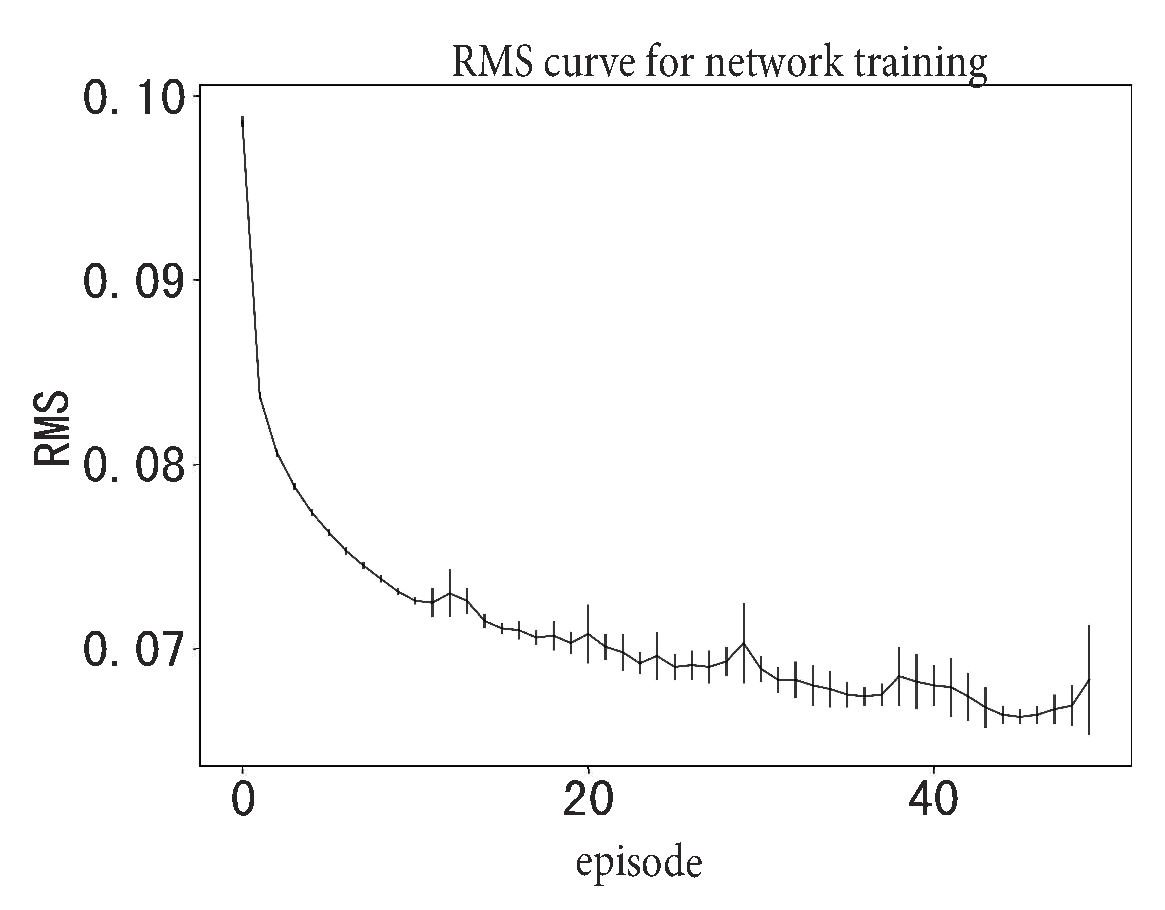
\includegraphics[width=\columnwidth]{Learning_curve}
\caption{Learning curve for SRNN}
\label{Learning curve for SRNN}
\end{figure}

Figure \ref{Learning curve for SRNN} shows the learning curve of SRNN, that is the change of 
RMS with the number of iterations. The data in the figure is the 
result of repeating 10 training sessions. 
It can be seen from the figure that the value of RMS 
gradually decreases with the number of iterations. 
It converges after about 15 iterations, which indicates that the training 
speed of SRNN is faster.

\begin{figure*}[htbp]
\centering
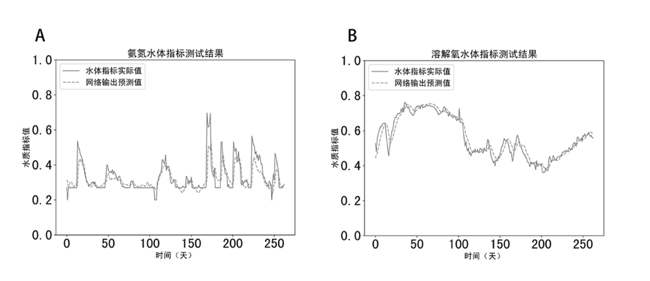
\includegraphics[width=\columnwidth]{Prediction_results}
\caption{Prediction results for ammonia and dissolved oxygen using SRNN}
\label{Prediction results for ammonia and dissolved oxygen using SRNN}
\end{figure*}

Although the SRNN training converges faster, it is necessary to 
calculate the prediction result of SRNN under the test data in 
order to characterize the prediction ability of SRNN. 
We test the prediction results of SRNN on 
ammonia nitrogen and dissolved oxygen in water quality. 
The predicted result is shown in Figure \ref{Prediction results for ammonia and dissolved oxygen using SRNN}. The solid line 
is the measured data of ammonia nitrogen and dissolved oxygen, 
while the dotted line is the predicted result given by SRNN. 
Ammonia nitrogen refers to nitrogen in the form of free ammonia 
($NH_3$) and ammonium ions ($NH_4^+$) in water. The ammonia nitrogen 
wastewater is mainly derived from chemical fertilizer, coking, 
petrochemical, pharmaceutical, food, landfill and so on. 
The discharge of a large amount of ammonia nitrogen wastewater 
into the water not only causes eutrophication of the water, 
but also causes black odor in the water.
The trend of the change of ammonia nitrogen in time in Figure 3 
indicates (solid line) that the change of ammonia nitrogen in water 
is extremely unstable and there are often mutations. 
The dissolved oxygen content in the water is closely related to
the partial pressure of oxygen in the air and the 
temperature of the water. Compared with the ammonia nitrogen 
index in water, the change of dissolved oxygen index 
is relatively flat. It is not difficult to find from the prediction 
results in Figure \ref{Prediction results for ammonia and dissolved oxygen using SRNN} 
(dashed line) that SRNN can accurately predict 
these two water quality indicators whether it is for the 
ammonia nitrogen index with mutation (Figure \ref{Prediction results 
for ammonia and dissolved oxygen using SRNN}(A)) or 
for the relatively stable dissolved oxygen 
(Figure \ref{Prediction results for ammonia and dissolved oxygen using SRNN}(B)). 
The prediction errors (RMS) for the two water quality 
indicators in Figure \ref{Prediction results for ammonia and dissolved 
oxygen using SRNN} against the test data set were 0.065 and 0.057.

Determining the model prediction results are often free parameters in the model, 
such as the number of BP network hidden layer neurons as well as the initial
value of the weight and the strength coefficient g of the SRNN recursive 
layer weight. The generalization ability of the SRNN network is verified
by calculating the RMS under repeated tests. 
Let the intensity coefficient g be equal to 0.5, 1.0 as well as 1.5 and run 10 
replicates for each parameter. Each repeated experiment includes two
phases of training and testing. The weight of each repeated experiment 
SRNN is randomly selected according to a given distribution. 
As shown in Figure \ref{Generalization for SRNN}(A), the mean values of the test
RMS under the three intensity coefficients are less 
than 0.08. Their respective variances are 0.0042, 0.0001 and 0.0006. This 
shows that SRNN can obtain better prediction results under different weight
intensity coefficients. In particular, when the intensity coefficient
$g$ is equal to 1.5, the spontaneous activity of the SRNN recursive network has
chaotic characteristics \cite{RN17}. But SRNN can still obtain better prediction results.

\begin{figure*}[htbp]
\centering
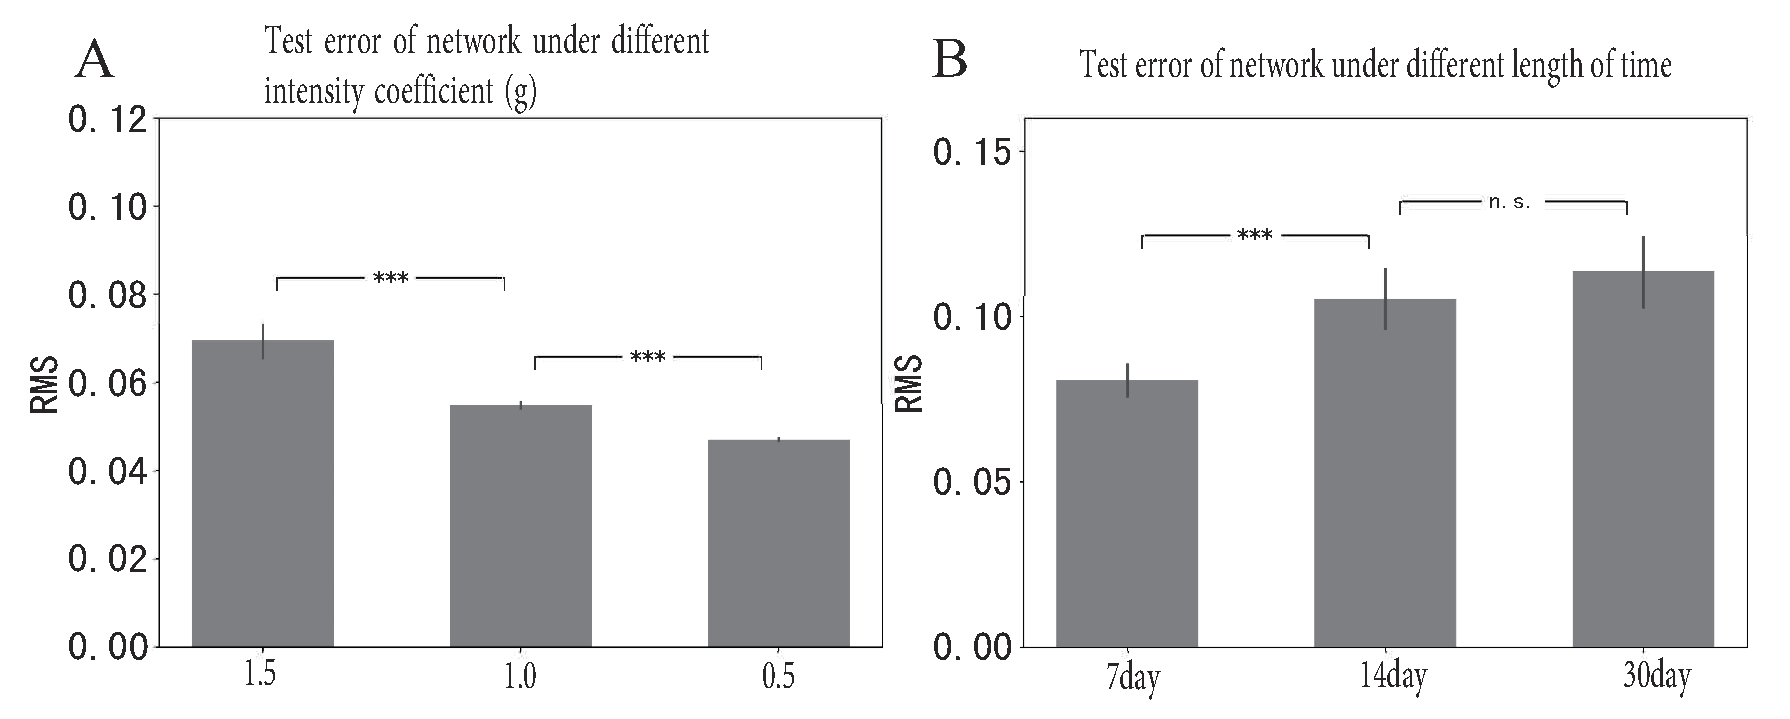
\includegraphics[width=\columnwidth]{Generalization_for_SRNN}
\caption{Generalization for SRNN}
\label{Generalization for SRNN}
\end{figure*}

The length of the SRNN input sequence has a different impact on the prediction results. 
As shown in Figure \ref{Generalization for SRNN}(B), the prediction 
results based on the time series of the 
previous 7 days are significantly better than the prediction results 
based on the time series of the first 14 days or the first 30 days.

In addition, SRNN was used to test the three water quality indicators of 
permanganate index, total nitrogen and total phosphorus in water. 
The test results are shown in Figure \ref{Prediction results for other water quality indicators}. 
It is not difficult to see that 
SRNN's predictions for these three water quality indicators are equally accurate.
\begin{figure*}[htbp]
\centering
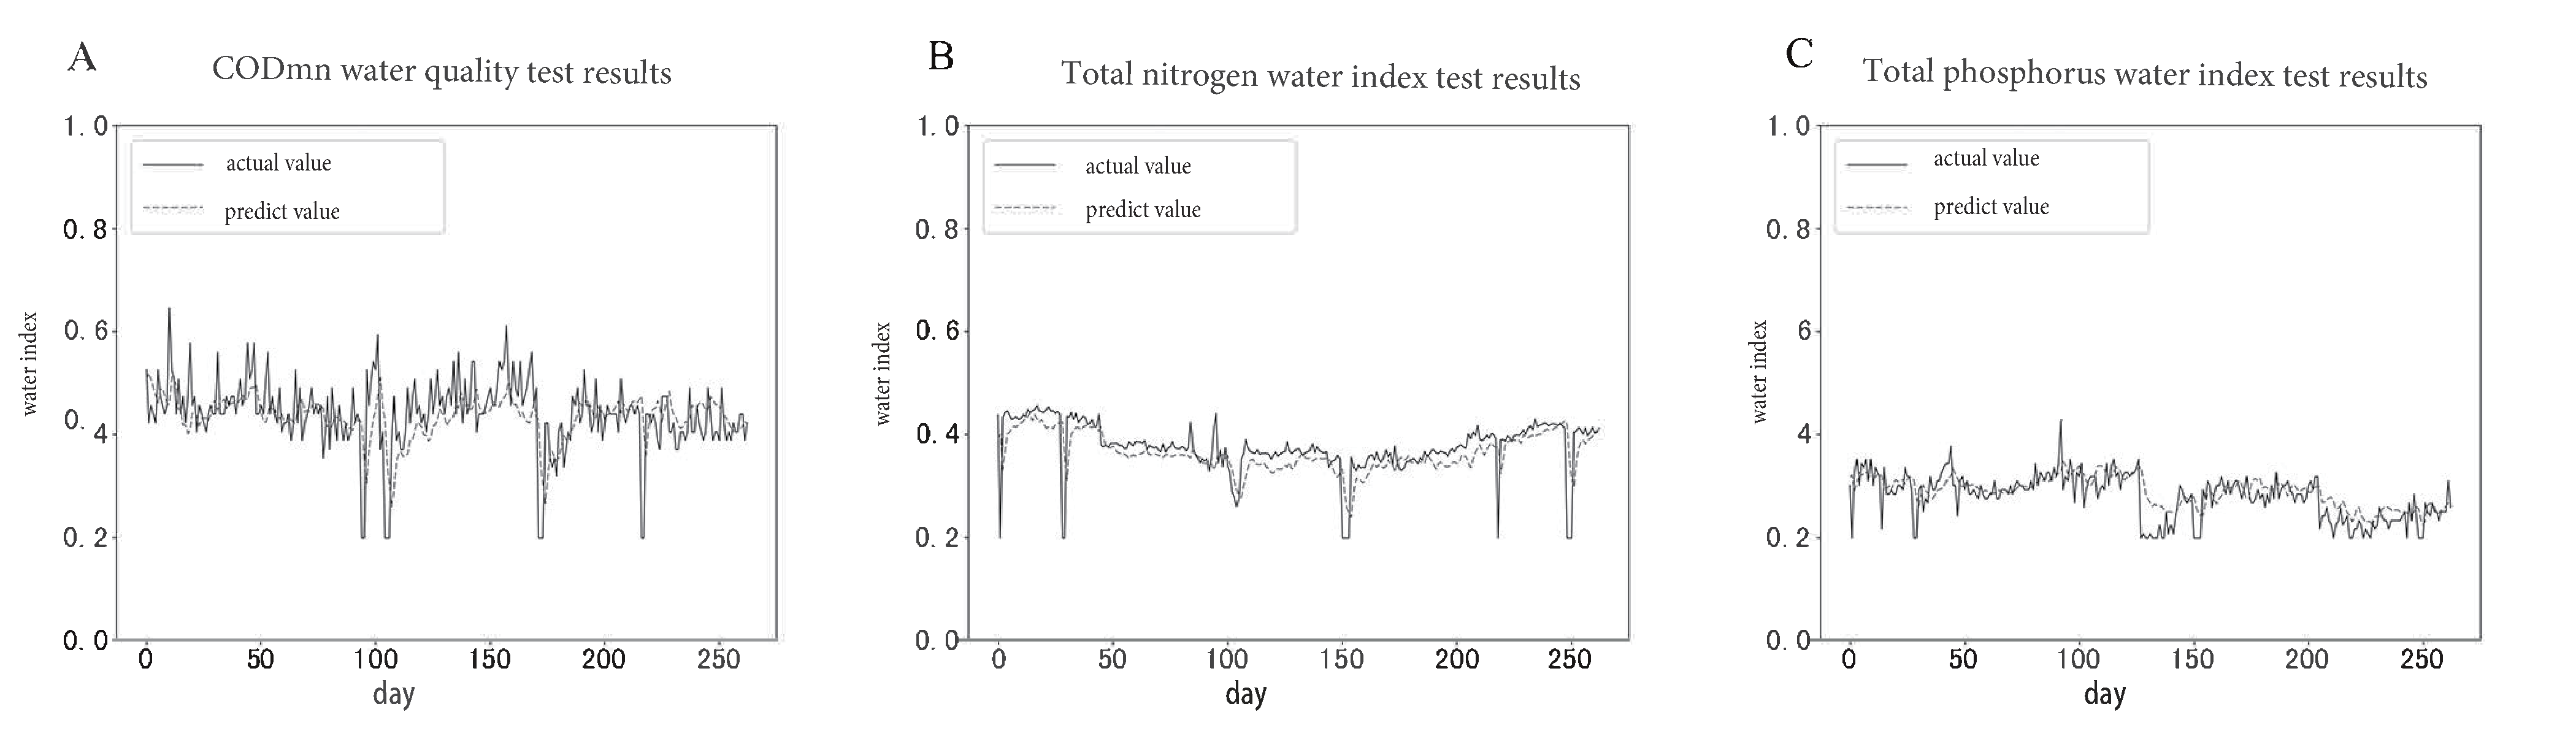
\includegraphics[width=\columnwidth]{Prediction_results_for_other_water_quality_indicators}
\caption{Prediction results for other water quality indicators}
\label{Prediction results for other water quality indicators}
\end{figure*}

\subsection{Water quality level prediction}
After successfully predicting water quality indicators, 
SRNN will be further used to predict water quality levels. 
According to the National Surface Water Environmental Quality Standard (GB3838-2002): 
the surface water quality grade (L) is divided into 
five grades from I to V. Class I-III water meets urban drinking water standards. 
In order to correspond to the five levels of water quality, the output of 
SRNN is modified to 5 neurons. Each neuron corresponds to a level. 
The five neurons with the highest rate of release are set to the output of SRNN:

\begin{equation}
L=argmax_i[z_1,z_2,z_3,z_4,z_5 ](i=1,2,3,4,5)
\end{equation}

When the output result $z = [0.001, 0.089, 0.2, 1.23, 0.5]^T$ and the index $i$ of 
the largest element in $z$ is 4, then the water quality level $L$ predicted by SRNN is IV. 
In order to more accurately describe the relationship between the predicted 
level and the true level, the relative distance $D$ between the two levels 
is also calculated to represent $e(t)$. The setting of $e(t)$ is shown in Table \ref{Training error setting}.
\begin{table}[htbp] 
\centering
\caption{Training error setting}
\label{Training error setting}
\begin{tabular}{cccccc} 
\toprule 
D&0&1&2&3&4\\ 
\midrule 
$e(t)$&0&0.15&0.25&0.35&0.45\\ 
\bottomrule 
\end{tabular} 
\end{table}

We use a total of 368 data sets with a 7-day monitoring interval from May 1,
2012 to April 30, 2014 during training process. We use a total of 200 data sets with a 
7-day monitoring interval from May 1, 2014 to April 30, 2015 during testing process. 
Through 20 repeated experiments, the best correct rate of water level prediction was $89\%$,
as well as the average correct rate was $85.6\%$. At the same time, 
this study also tests the SRNN forecast to reach the water quality
level in the next 2 to 6 days.  As shown in Figure \ref{Predict water quality level using SRNN}, the correct rate of prediction 
results is above $80\%$.

\begin{figure}[htbp]
\centering
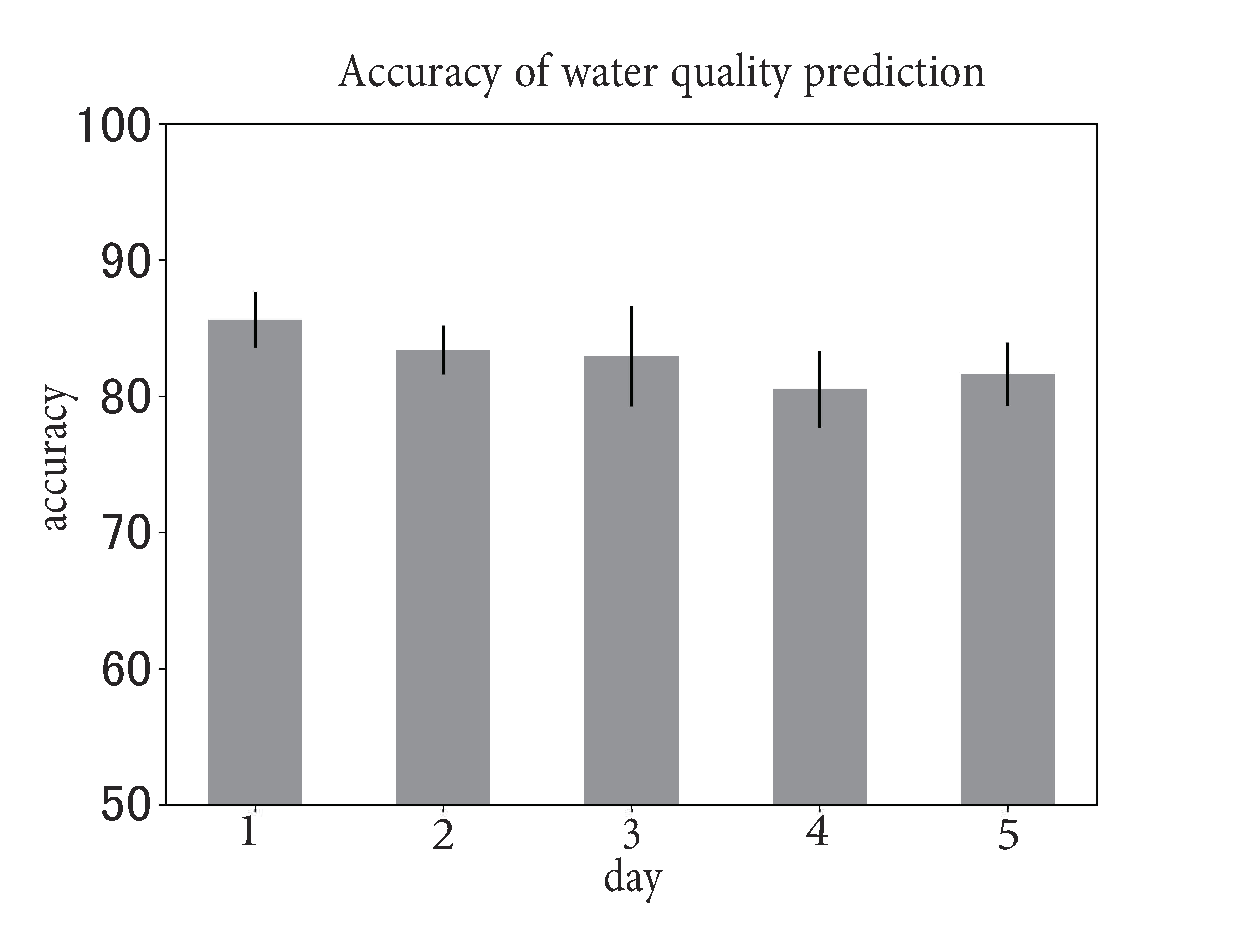
\includegraphics[width=\columnwidth]{Predict_water_quality}
\caption{Predict water quality level using SRNN}
\label{Predict water quality level using SRNN}
\end{figure}

\subsection{Model comparison}
The effectiveness of SRNN has been demonstrated by predicting 
different water quality indicators and water quality levels in a river. 
In the following, we will further explain that SRNN is more suitable 
for the prediction of water quality indicators and grades with time 
correlation by comparing with the prediction results of BP neural network. 
BP neural network model structure is a three-layer structure BP. The number 
of neurons in the input layer corresponds to the input length of the data. 
The time scale of the input data is converted together into the input of 
the BP network. The number of hidden layer neurons is taken as 13, 
and the number of neurons in the output layer is set to 1 or 5 according 
to the prediction task. The experiment was repeated 10 times. 
The comparison between the BP network and the SRNN prediction results is shown in Table 
\ref{Comparison on prediction results between BP network and SRNN network}.

\begin{table*}[htbp] 
\centering
\caption{Comparison on prediction results between BP network and SRNN network}
\label{Comparison on prediction results between BP network and SRNN network}
\begin{tabular}{ccccccc} 
\toprule 
\multirow{2}{*}{model}&\multicolumn{5}{c}{RMS error value}&\multirow{2}{4.25cm}{Accuracy of next day}\\
\cline{2-6}
&AN &DO&PI&TP&TN&\\
\midrule 
SRNN&0.0342&0.0234&0.0468&0.0241&0.0244&$85.6\%$\\
BP&0.066&0.1082&0.0943&0.0441&0.0662&$51.75\%$\\
\bottomrule 
\end{tabular} 
\end{table*}

\section{Discussion}
In this study, a recurrent neural network with sparse connection features was 
designed to model the water quality data. The mean square recursive error algorithm 
was used to train the network to predict various indicators of water quality 
and water quality levels. The simulation results show that SRNN has better 
prediction ability. In particular, SRNN has few free parameters. The three 
weights of $w^{RNL}$, $w^{in}$, and $w^{fb}$ only need to be randomly set 
according to the distribution to obtain better prediction results.
This makes SRNN easier to apply to environmentally variable water 
quality predictions.

SRNN which is similar to Echo State Network (ESN) training only needs 
to adjust the weight between recursive layer and output layer. 
This greatly improves the operational efficiency of the recursive network. 
Since there is no need to adjust the connection weights between the neurons 
in the recursive layer during learning, the recursive layer of SRNN 
and ESN can be considered as a general-purpose computing unit similar
 to the function of the prefrontal cortex of the brain\cite{RN20,RN21}. 
 Although SRNN and ESN are similar in structure, there are also essential 
 differences between them. Firstly, SRNN's recursive layer connection 
 weight does not require special settings. In order to achieve 
 reverberation, ESN requires a weight matrix with a spectral radius 
 greater than or equal to 1. Secondly, ESN training is a kind of 
 offline learning, that is, it needs to wait for the network to 
 pre-calculate for a period of time before adjusting the output 
 weight. But SRNN can update the output weights on the fly based 
 on the current input. This feature is especially important 
 in situations where the amount of training data is insufficient. 

 The good predictive performance of SRNN is not only related to 
 its structure, but also closely related to the learning algorithm 
 it uses. It is not difficult to see from Equation 5 and 6 that the 
 learning algorithm of SRNN is the same as the BP network error 
 back propagation algorithm. However, compared to the error 
 backpropagation algorithm, the learning process of SRNN can 
 quickly make the network output close to the target output 
 which mainly in the calculation of the matrix $P$. The matrix $P$ 
 is equivalent to the inverse of the correlation matrix in 
 estimating the recurrence rate of the recursive layer \cite{RN23}. 
 Intuitively, SRNN's algorithm can accurately adjust the weights 
 between the neurons and the output neurons based on the activity 
 of the recursive layer neurons, so that the output of the 
 output neurons quickly approaches the actual output value. 
 In addition, SRNN has better predictive performance than BP 
 networks commonly used for water quality prediction. Because 
 the BP network is just a feedforward neural network, which 
 cannot model the correlations that may exist in the input data 
 over time. SRNN which is unlike BP networks is a recurrent neural 
 network. The existence of the recursive layer makes it possible 
 to establish the temporal correlation of the input data. 

The prediction model proposed in this study belongs to the 
data-driven water quality prediction model DDM. Compared with
PDM, DDM can adapt to water quality prediction under changing 
conditions. However, the model constructed in DDM mode is 
difficult to interpret from the perspective of true biochemical 
reaction between water quality indicators. This makes it possible
to overfit the data when applying DDM. Therefore, when applied to 
the prediction of water quality indicators, considering the integration 
of PDM into DDM is a problem that needs to be studied in the future.
In addition, there are many factors affecting water quality parameters 
and grades, such as seasons and climate. However, this study did not add 
these factors to the model. Therefore, how to integrate more variables 
into SRNN to improve the accuracy of model prediction is a problem 
worthy of further study.  

\section{Conclusion}
This study designed a recurrent neural network with sparse
connection features for modeling water quality data. 
This study uses the mean square recursive error algorithm 
to train the network to predict various indicators of water 
quality and water quality levels. The simulation results 
show that the method has the characteristics of wide 
adaptability to the model parameters and fast convergence.
This method can be used to predict the future trends of
water quality parameters and water quality levels of 
rivers and lakes. The method can play an active role 
in intelligent modeling of river water quality, 
watershed planning and pollution control.
%
% ---- Bibliography ----
%
% BibTeX users should specify bibliography style 'splncs04'.
% References will then be sorted and formatted in the correct style.
%
 \bibliographystyle{splncs04}
 \bibliography{mybibliography}

\end{document}
